\documentclass[a4paper]{article}

\usepackage[english]{babel}
\usepackage[utf8]{inputenc}
\usepackage{mathtools}
\usepackage{gensymb}
\usepackage{amssymb}
\usepackage{amsmath}
\usepackage[thmmarks,amsmath]{ntheorem}
\usepackage{booktabs,siunitx}
\usepackage{graphicx}
\usepackage[colorinlistoftodos]{todonotes}
\usepackage{geometry}
\usepackage{float}
\usepackage{hyperref}
\usepackage{caption}
\usepackage[bottom]{footmisc}
\geometry{
 a4paper,
 total={170mm,257mm},
 left=30mm,
 right=30mm,
 top=20mm,
}
\author{[[Name]]}
\title{Report - [[Experiment]]}

\begin{document}

\maketitle
\abstract 

The main task of the following report is to verify the exponent of $-4$ of the sinus expression in the famous Rutherford scattering formula

\begin{equation}
\sigma(\theta) = \frac{d\sigma(\theta)}{d\Omega} = \left( \frac{Z_1 Z_2 \epsilon^2}{4E} \right)^2 \frac{1}{\sin^4{\theta / 2}}.
\end{equation}

It was calculated from the measured data to be $[[a]]$ which strengthens the model. This leads to the conclusion that the atomic cores in the center of the atom are responsible for the scattering. Therefore the Rutherford model of the atom was derived, which says that the nucleus of the atom is very concentrated in a small volume, whereas the electrons are far away compared to the radius of the nucleus.

\section{Introduction}

In 1904 J.J Thompson proposed the first atomic model, to which many will follow. It stated that the negatively charged electron occupies a region of space in the atom which is of uniform positive charge and shaped as a sphere. Between 1908 and 1913 there was a series of experiments known as the Geiger-Marsden experiments, which disproved the Thompson model. These were directed by Ernest Rutherford. As a significant consequence Rutherford later derived a model for the structure of the atom, where the positive charge and the bulk of the mass is highly concentrated in the center of the atom. The electron on the other side orbits around the center in a radius huge compared to the radius of the so called nucleus - the positive chaged core. This suggests that in the atom there is much empty space.
\newline

\subsection{Rutherford scattering}
\label{sec:rutherford}

Rutherford derived his model for the atom in 1911, based on elastic scattering of a particle at the core. This replusion is assumed to be caused from a Coulomb potential near the atom core, hence within the shielding of the electrons and therefore of negligible deflection trough the electrons. The deflection must thus be caused by the nucleus. He came up with the following famous scattering formula:

\begin{equation}
\sigma(\theta) = \frac{d\sigma(\theta)}{d\Omega} = \left( \frac{Z_1 Z_2 \epsilon^2}{4E} \right)^2 \frac{1}{\sin^4{\theta / 2}}.
\label{eq:rutherford}
\end{equation}

where $\sigma$ is the cross section. It is assumed that the target thickness is very small such that the cross ection if two neighboring target atoms will never overlap. $\frac{d\sigma(\theta)}{d\Omega}$ is called the differential cross section, where $d\sigma$ is the differential size of the cross section and $d\Omega$ is the differential solid angle. Thus the differential cross section describes the area per solid angle. $\theta$ is the angle relative to the beam (of $\alpha$-particles in case of this experiment). $Z_1$ is the charge of the $\alpha$-particle whereas $Z_2$ is the charge of the gold target atoms. The energy $E$ is the kinetic energy of the incoming $\alpha$-particle.

To get a formula of measurable quantities, we use that the probability of scattering at a target area $A$ is $W = \frac{N_a / t}{N_e / t} = \frac{N_{AK} \sigma}{A}$, which leads to the infinitesimal equation

\begin{align}
dW = \frac{d N_a / t}{N_e / t} = \frac{N_{AK} d\sigma}{A}
\label{eq:dprob}
\end{align}

where $N_a$ is the number of scattering events, $N_e$ is the number of incident paticles, $\sigma$ is the cross section and $N_{AK}$ is the number of atoms inside the target volume $V = A d$, with $A$ the area and $d$ the thickness. From this we get

\begin{align}
d N_a = \frac{N_{AK} N_e d \sigma}{A} = \frac{N_{AK} N_e}{A} \frac{d \sigma}{d \Omega} d \Omega
\label{eq:dNa}.
\end{align}

After integrating over the solid angle $\Omega_D$ of the detector, using that the activity of the source at the gold foil is $I_S = \frac{N_e}{t} \frac{\Omega_F}{4 \pi}$ and using Rutherford's formula \eqref{eq:rutherford}, we obtain the formula

\begin{equation}
\log{\left( \frac{N_a}{\Omega_D t} \right)} = \log{C} - 4 \log{\left( \sin{\frac{\theta}{2}} \right)}.
\label{eq:log}
\end{equation}

after taking the logarithm of both sides, where $C = n_{AK} d I_S \frac{\Omega_F}{4 \pi} \left( \frac{Z_1 Z_2 \epsilon^2}{4 E} \right)^2$, with $n_{AK} = \frac{N_{AK}}{A d}$. This is the Rutherford scattering formula considering the finite size of the detector. In the formula are only measurable or known quantities.

We are interested in the prefactor of $\log{\left( \sin{\frac{\theta}{2}} \right)}$ which should be $-4$ according to this model. If we plot $y = \log{\left( \frac{N_a}{\Omega_D t} \right)}$ against $x = \log{\left( \sin{\frac{\theta}{2}} \right)}$ and fit the measured values on a fitline $y = a x + b$, we should be able to determine the slope $a$ and the constant $b = \log{C}$.

\subsection{Stopping power}

Charged particles moving trough matter suffer loss of energy and a change of direction. This loss of energy depends on the velocity and charge of the particle and of the target material. When $\alpha$-particles move trough gold atoms, they perform inelastic collisions with the electron in the shell of the gold atom. The formula for electric energy loss per unit length (stopping power) was derived by Bethe and Bloch in 1932. The non-relativistic form is

\begin{equation}
-\frac{dE}{dx} = \frac{2 \pi Z_1^2 \epsilon^4}{E_{\alpha}} \frac{m_{\alpha}}{m_e} n_e \log{\left( \frac{4 E_{\alpha}}{<E_B> m_{\alpha} / m_e } - K\right)}
\label{eq:bethebloch}
\end{equation}

where $E_{\alpha}$ is the energy of the incoming $\alpha$-particle and $m_{\alpha}$ its mass, $m_e$ is the electron mass, $n_e$ is the electron density of the target, $<E_B>$ is the mean ionisation potential of the target and $K$ is a correction constant depending on the target material.

\subsection{Total energy loss}

With the above theory, an $\alpha$-particle will lose energy on its way from the source trough the gold foil and air to the detector. For concrete theoretical calculations please refer to section \ref{sec:energy_loss}.

\section{Setup}

\subsection{The apparatus}

The used apparatus is a cylindrical vacuum chamber where on one side there is a window for the source of the alpha particles and on the other side is a aperture for the detector. Inbetween them inside the pipe a ring-shaped gold foil is placed. An electric pump is attached to evacuate the chamber (see figure \ref{fig:setup}).

\begin{figure}[H]
\captionsetup{singlelinecheck=off}
\centering
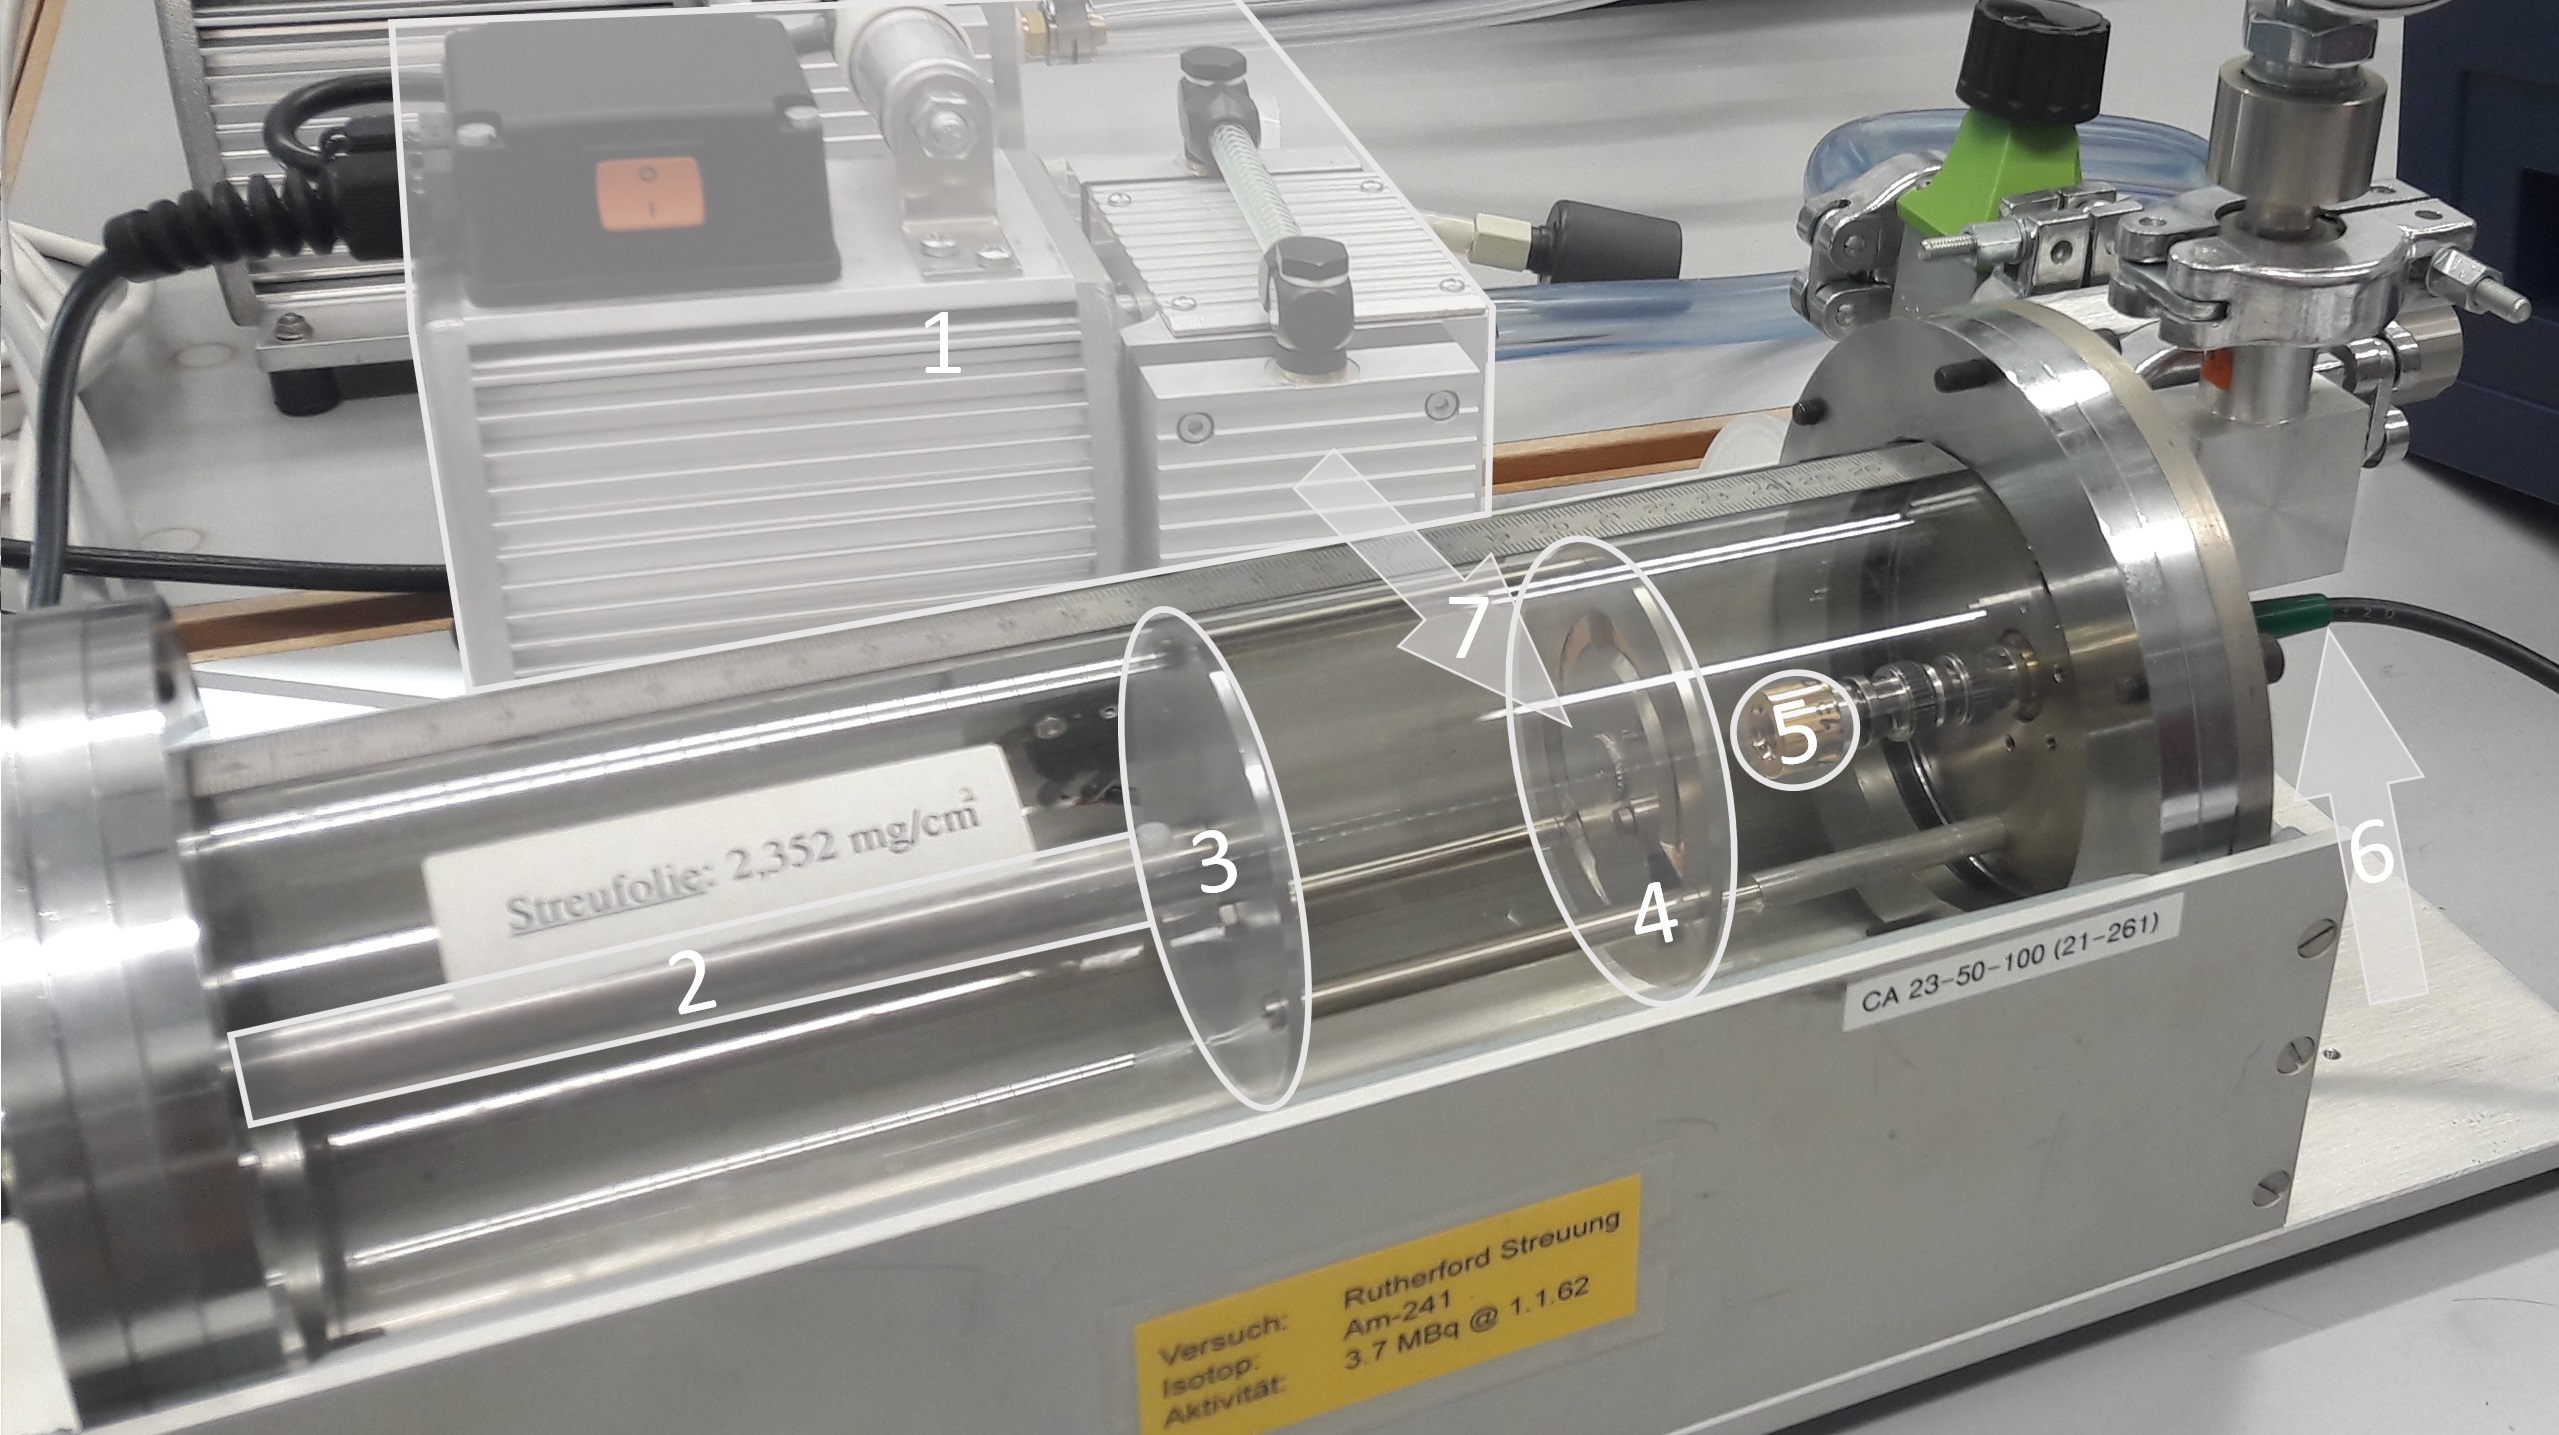
\includegraphics[width=1.0\textwidth]{img/setup.jpg}
\caption[blubb]{Image of the experimental setup. The cylindrical glass element is the vacuum tube. $1$ is the pump to evacuate the chamber, $2$ is the mechanic rod to adjust the distance of the source to the gold foil from outside the chamber, $3$ is the $^{241}Am$ source emitting the $\alpha$-particles, $4$ is the circle element with the gold foil ring, $5$ is the surface barrier nuclear particle detector, $6$ points to the cable leading from the detector to the preamplifier and $7$ points to the small aperture in the center of $4$. This aperture can be opened by turning the mechanic rod $2$. Source: Authors' own.}
\label{fig:setup}
\end{figure}

\subsubsection{The source}

The $\alpha$-source on the left side of the tube (see figure \ref{fig:geometry}) is mounted on a slidable rod to adjust the distance of the source and the gold foil (which is fixed $\delta$) to the detector from outside the vacuum chamber by hand. With this, the distance $x$ can be regulated from $\approx 2cm$ up to $\approx 20cm$. The source was an Americium-241 compound ($^{241}Am$) which decays in Neptunium-237 ($^{237}Np$) under emission of $\alpha$-particles. It has a half-life time of approximately $432.2$ years \cite{audi2003}.

\subsubsection{The foil}

The gold foil is positioned in the middle of the vacuum tube (see figure \ref{fig:geometry}). It is shaped in a circular ring one side facing the source and the other side facing the detector. The ring is filled with high density material blocking the $\alpha$-particles. The foil itself has a thickness of $[[d]] \mu m$. There is a mechanic rig to open a hole in the center such that the $\alpha$-particles can pass trough without scattering.

\subsubsection{The detector}

The detector mounted on the opposite side of the tube (see figure \ref{fig:geometry}) is a surface barrier nuclear particle detector which consists of a mono-crystal silicon with a thin gold film evaporated.

\begin{figure}[H]
\captionsetup{singlelinecheck=off}
\centering
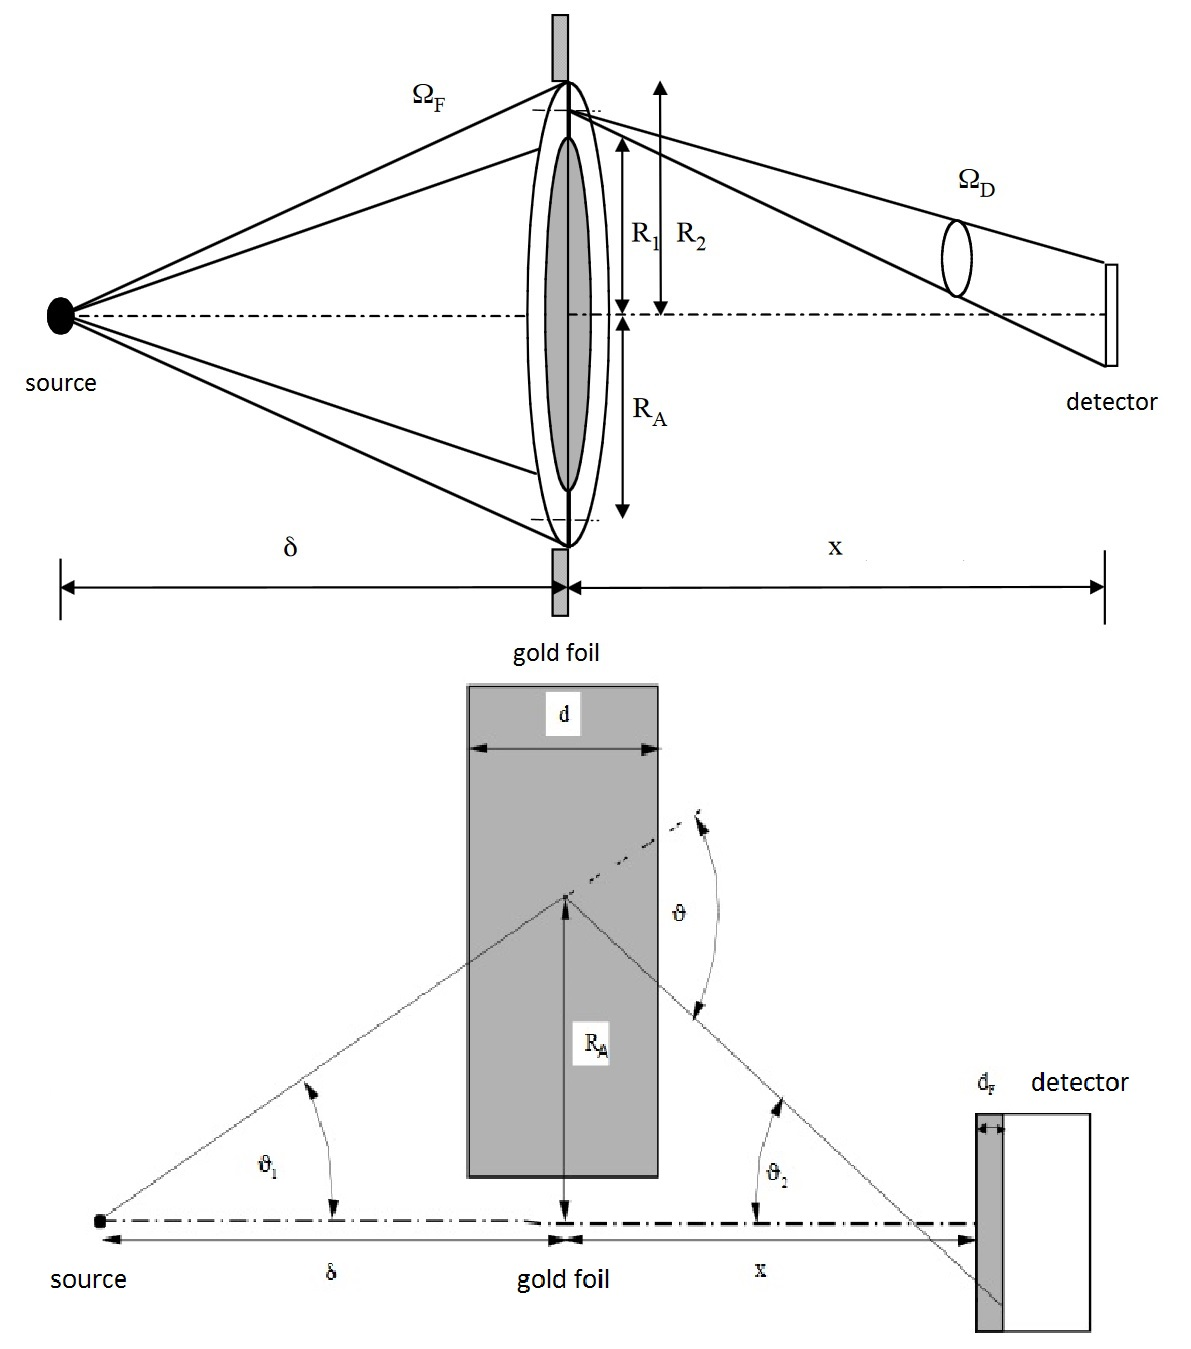
\includegraphics[width=0.7\textwidth]{img/geometry3.jpg}
\caption[blubb]{Scattering geometry. Upper: The source, the gold foil and the detector lie on a straight line. The white ring around the gray shaded region is the gold foil, where the scattering occures. $\Omega_F$ is the solid angle through which the sources sees the foil and $\Omega_D$ through which the foil sees the detector. Lower: Geometry of the foil part itself, the gray shaded part is the cross section of the gold foil, $d$, $d_F$ are the thickness of the foil and the distance to the detector surface. Source: Instruction sheet \cite{inst2007}.}
\label{fig:geometry}
\end{figure}

\subsection{Subsecquent processing}

The detector gives a charge impulse signal which is intensified by the preamplifier that gives a voltage impulse signal. The dicriminator attached to the preamplifier generates a signal form in a rectangular pattern of height propartional to the enery of the $\alpha$-particle approaching the detector in the first place. These unit pulses are counted by a TTL-counter. The discriminator is set up, such that only relevant peaks are counted (see section \ref{sec:operating_point}).

\section{Measurements and Discussion}

\subsection{Evacuation of the scattering camber}

The first task was to evacuate the scattering chamber with an electronic pump. It was evacuated to a pressure of $[[pressure]] \, mbar$.

\subsection{Discriminator Curve}

Before measuring the angle distribution, the discriminator device had to be set up correctly. For this, the middle hole needed to be open. The detected $\alpha$-particles were counted and the time was stopped, while the potentiometer was turned step by step, until the device was adjusted, such that no $\alpha$-particle hit the detector anymore. This was done in steps of $0.5$ turns, until the discriminator started to detect less $\alpha$-particles, than before (see figure \ref{fig:discriminatorCurve}). From around $3.5$ turns away, the we reduced the step size to $0.25$ to get more data in the relevant sections of the curve.

The derivative of the error function fit in figure \ref{fig:discriminatorCurve} is

\begin{equation}
f'(x) = \frac{2 a b e^{-(b x + c)^2}}{\sqrt{\pi}}
\label{eq:gaussian}
\end{equation}.

This is the pulse height spectrum.

\subsubsection{Operating point / Discriminator setting}
\label{sec:operating_point}

The operating point of the dicriminator device was chosen to be $1$ turn (see figure \ref{fig:discriminatorCurve}) after some analysis of the discriminator curve. The operating point should be set before the downward slope of the discriminator curve, such that the device won't prevent relevant $\alpha$-particles in the peak of the pulse height spectrum to approach the detector.

\subsubsection{Activity - Part 1}

To obtain the activity of the source, the mechanical rod on the tube was set to the shortest distance achievable with the experimental setup and the middle gap was opened. It was chosen to be $x_{act} = [[x_activity]] \, cm$. With this set, we measured $N = [[counts_activity]]$ counts in $t = [[seconds_activity]]$ seconds, leading to $N/t = [[rate_activity]]$ counts per seconds.
\newline
Those measured quantities give an approximate activity of the source of

\begin{align}
I_{S,1} = \frac{N}{t} \frac{4 \pi}{\Omega_{g}} &= [[I_S1MBq]]\, MBq \label{eq:activity1} \\
&= [[I_S1muCi]] \, \mu Ci
\end{align}

where $\Omega_g$ is the solid angle of the gap (and the detector). Since $\frac{A_g}{\delta^2} < \frac{A_D}{\left( \delta + x_{act}\right)^2}$, the correct value for $\Omega_g$ is $\frac{A_g}{\delta^2}$, where $A_g$ is the area of the gap ($A_D$ is the sensible area of the detector). Since the nominal activity of the source was $[[I_then]]$ MBq in january $1$ $1962$, we see that the measured quantities give an activity which is lower than that. This makes sense, because the activity falls exponentially according to the law of radioactive decay. The calculated value of the activity according to the law of radioactive decay is

\begin{equation}
I_{S,calc} = [[I_now_radl]]\, MBq. \label{eq:activity:calc} \\
\end{equation}

This values is very close to $I_{S,1}$.

\begin{figure}[H]
\centering
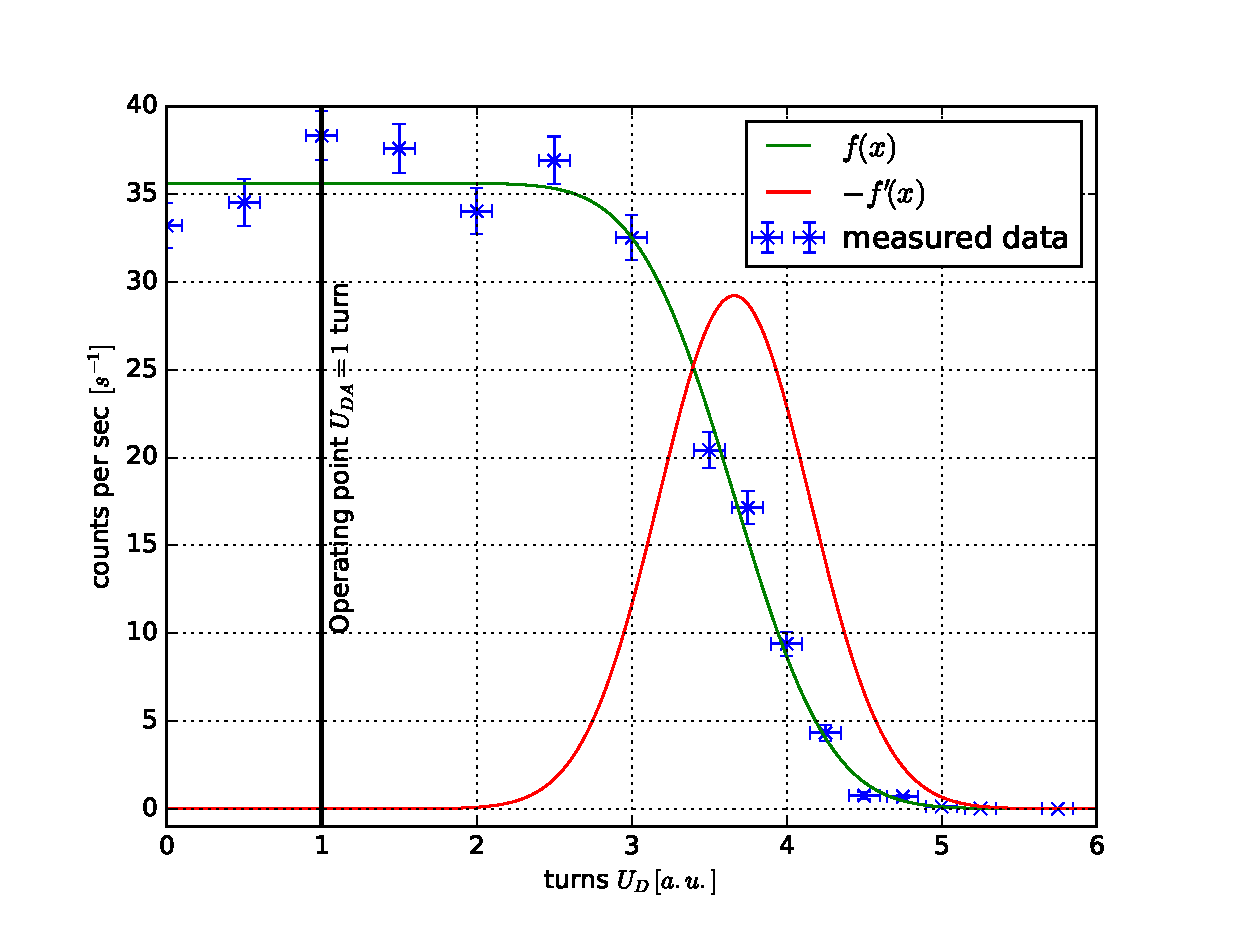
\includegraphics[width=1.0\textwidth]{plots/discriminator_curve.eps}
\caption{Discriminator curve and its error function fit $f(x)$. The parameters for the fit curve are as follows: $f(x) = a \cdot erf(b \cdot x + c) + d$ with $a = [[fit:erf_a]]$, $b = [[fit:erf_b]]$, $c = [[fit:erf_c]]$ and $d = [[fit:erf_d]]$. This looks like the complementary error function $erfc() = 1 - erf()$, but nonetheless the above fitting parameters ($a$ to $d$) are for the error function as stated in the model, not its complementary. The operating point $U_{DA}$ is set to $1$ turn. $f'(x)$ is the pulse height spectrum. Source: Authors' own.}
\label{fig:discriminatorCurve}
\end{figure}

\subsection{Angle distribution}

In figure \ref{fig:angleDistribution2} the angle distribution is plotted against the angle $\theta$. It can be seen that for smaller angles $\theta$ the counts per second into the solid angle of the detector ($\Omega_D$) increase. This is expected, because since $\theta = \theta_1 + \theta_2$ and this is minimal, when both $\theta_1$ and $\theta_2$ are minimal. This means that we see more $\alpha$-particles scattering through the lower half of the gold foil with smaller angles that through the upper half with bigger angles (see figure \ref{fig:geometry}). It is expected that the higher the angle $\theta$ becomes, the less $\alpha$-particles will approach the detector and with angle $\theta_2 = \frac{\pi}{2}$ (when the detector and the gold foil are at the same position) the detector will see only forwardscattered particles.

\begin{figure}[H]
\centering
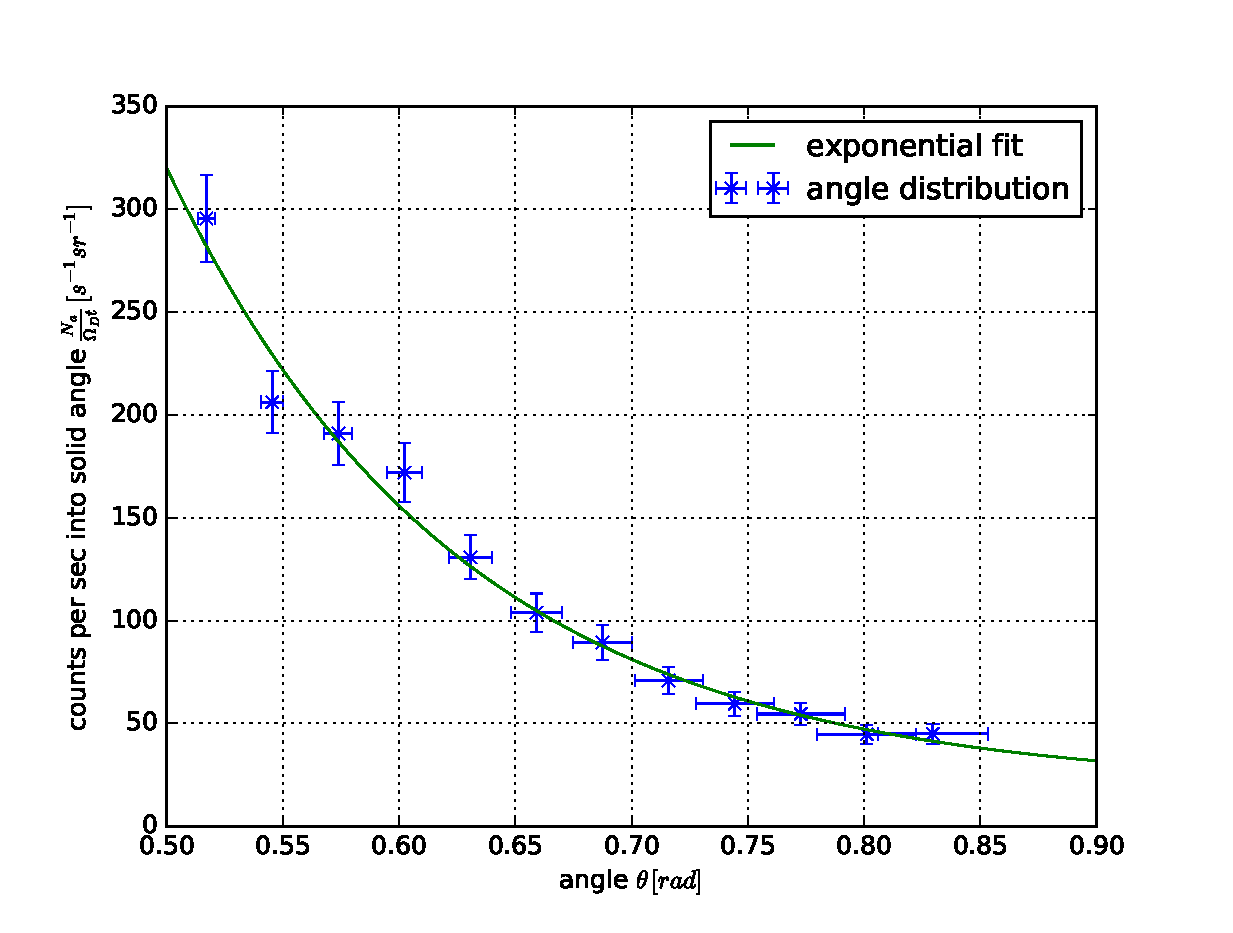
\includegraphics[width=1.0\textwidth]{plots/angle_distribution2.eps}
\caption{Angle distribution. The counts per second into solid angle of the detector $\Omega_D$ are poltted against the angle $\theta = \theta_1 + \theta_2$. The parameters for the exponential fit curve are as follows: $f(x) = a \cdot exp(b \cdot x + c) + d$ with $a = [[fit:exp_a]]$, $b = [[fit:exp_b]]$, $c = [[fit:exp_c]]$ and $d = [[fit:exp_d]]$. Source: Authors' own.}
\label{fig:angleDistribution2}
\end{figure}

\subsubsection{Underground}

The underground was measured with the source and the middle gap closed. As a result after more than $30$ minutes of measuring, no underground was determined. Therefore no adjustment of the measured data is needed.

\subsubsection{The exponent $a = -4$}

Figure \ref{fig:angleDistribution} shows the measured data and the calculated $\theta$ as of equation \eqref{eq:log} as $y = a x + b$; the regression line. From this plot we can finally read off the value of $a$, which is the exponent of $\sin{\frac{\theta}{2}}$ in the Rutherfold formula. The value of $a$ was obtained to be $a_{meas} = [[a]]$ and the value of $C$ to be $C = e^b = [[C]]$.
\newline
Since $a$ is very close to its theoretocal value of $a_{theo} = -4$, the experiment verifies Rutherford's scattering formula and thus the atomic model, where the positive charge is concentrated in a small region in the center of the atom.

\begin{figure}[H]
\centering
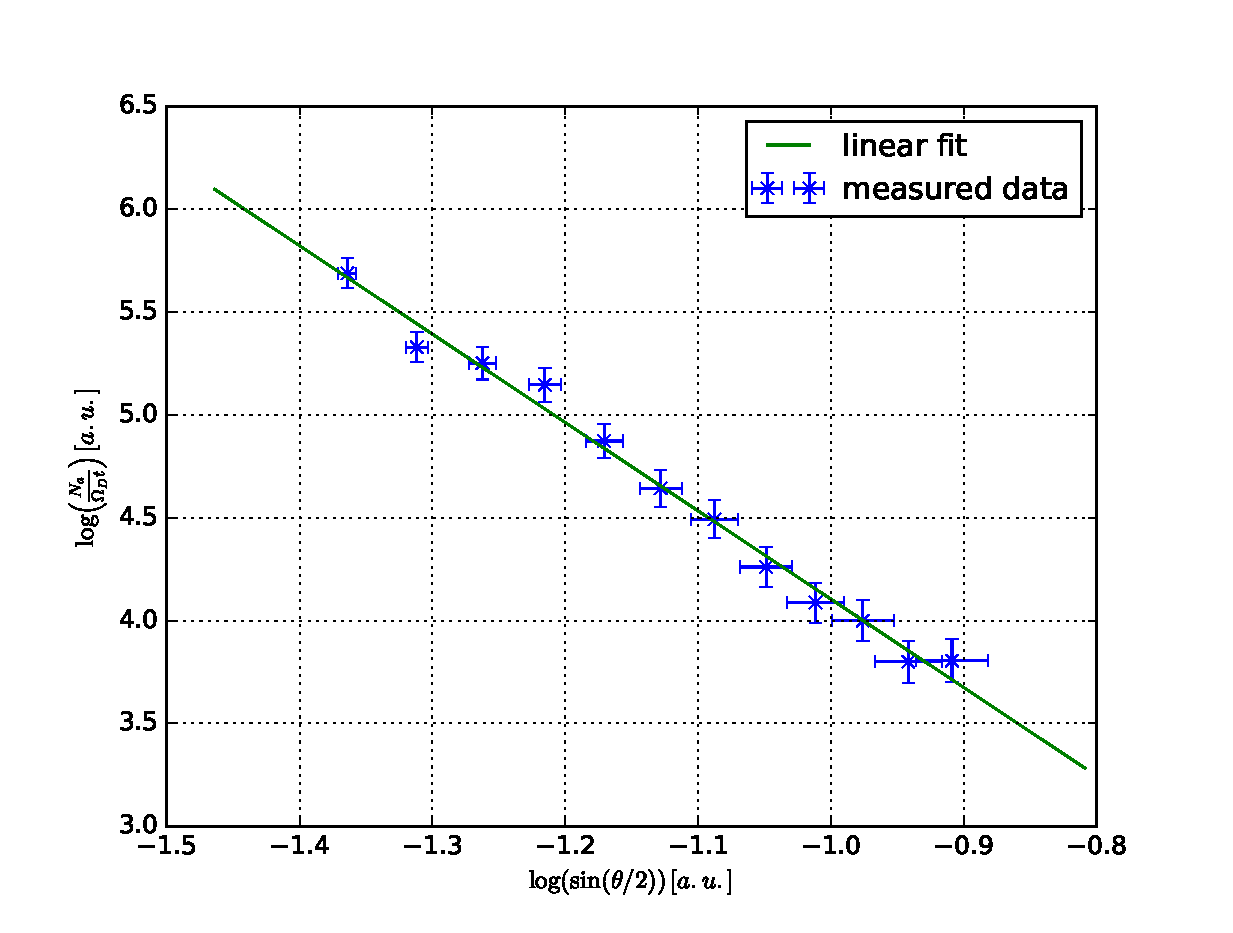
\includegraphics[width=1.0\textwidth]{plots/angle_distribution.eps}
\caption{Angle distribution. The parameters for the linear fit curve are as follows: $f(x) = [[linearFit]]$. Source: Authors' own.}
\label{fig:angleDistribution}
\end{figure}

\subsubsection{Activity - Part 2}

With the value of $C$, it is possible to calculate the activity of the source $I_S$ one more time, since all other quantities are known. From the theory in section \ref{sec:rutherford}, solved for $I_S$ we get:

\begin{equation}
I_S = \frac{4 \pi C}{n_{AK} \Omega_F d} \left( \frac{4 E}{Z_1 Z_2 \epsilon^2} \right)^2
\end{equation}

where $n_{AK}$ is number density of the target atoms, $\Omega_F$ is the solid angle and $d$ the thickness of the gold foil. The activity is then calculated to be

\begin{equation}
I_{S,2} = [[I_S2MBq]] \, MBq. \label{eq:activity2}
\end{equation}

This value is in the order of magnitude of the first calculation of $I_{S,1}$ (see equation \eqref{eq:activity1}). The formula above gives just for a rough estimation of the intensity. This lies on the value of $C$, which is $e^b$, where $b$ is from the linear fit $a x + b$ of the measured data (see figure \ref{fig:angleDistribution}). Since all measured data points are concentrated far away from $x = 0$, $b$ has a large uncertainty: $[[fit:b]]$.

\subsubsection{$\chi^2$-Test}

According to the $\chi^2$-Test, the value of $\chi^2 = S = [[chi_sq]]$, which then gives for the reduced $\chi^2$

\begin{equation}
\chi_r^2 = \frac{S}{\nu} = [[chi_r_sq]] < 1.
\end{equation}

$\chi_r^2$ is very close to $1$, but $<1$. This suggests that the linear interpolation of the data is justified and the quality of the measurement is sufiicient. This leads to a probability of error of $\alpha = [[alpha]] \, \%$ accoring to table $A1$ from the instruction sheet \cite{inst2007}. The table was linearly interpolated for al values of $\alpha$ in the row $\nu = 10$.

\subsection{Errors}

In this experiment there were 4 quantities that were measured: the number of $\alpha$-particles hitting the detector ($counts$), the time it took ($t$), the turn of the potentiometer for the operation point ($turns$) and the distance of the gold foil to the detector ($x$).

\begin{itemize}
\item The error for $n$ counts was calculated to be the $\Delta counts = \sqrt{n}$.
\item The time was taken by hand with an electronic stopwatch. The error that chosen to be $\Delta t = [[time_readoff_error]] \, s$.
\item Turning the potentiometer was also done manually. The error therefore was chosen to be $\Delta turns = [[delta_turns]] \, turns$.
\item The distance to the detector was set by hand with the mechanical rod. The readoff error for $x$ was chosen to be $\Delta x = [[x_readoff_error]] \, cm$, because one had to align the scale on the tube and the distance of the gold foil by eye.
\end{itemize}

\subsection{Systematic error sources}
\label{sec:systematic_errors}

In this experiment there are some sources of systematic errors that were ignored.

\begin{itemize}
\item The gold foil is assumed to be thin, such that no two cross sections of two neighboring gold atoms will overlap.
\item The Rutherford scatter formula \eqref{eq:rutherford} was derived using the Coulomb potential between two particles of charge $Z_1 e$ and $Z_2 e$ respectively. With this no shielding of the core charge through the electron shell is assumed. There might be small deflection due to interaction with the electrons in the shell.
\item In the trajectories of the $\alpha$-particles in air (from the source to the gold foil and from the gold foil to the detector), there is no energy loss assumed through collisions with molecules in the air. This simplification can be justifyed with the calculations in section \ref{sec:energy_loss} (equation \eqref{eq:loss_in_air}).
\item The tajectories of the $\alpha$-particles were simplified in a way that the particles will penetrate the gold foil in the center, whereas the source emits them distributed over all directions. As seen in the calculations in section \label{sec:crosssection}, the corrections in the cross section of $\theta_{min}$ and $\theta_{max}$ are different in the center of mass system of the gold atoms compared to the lab frame. Also they differ highly for the minimal and maximal angle $\theta_{min}$ and $\theta_{max}$. This leads to a systematic error in the calculation of the cross section $\Omega_D$ in which the radius $R_A = \frac{1}{2} \left( R_1 + R_2 \right)$ (see figure \ref{fig:geometry}) was used.
\item In section \ref{sec:energy_loss} in equations \eqref{eq:e_min} and \eqref{eq:e_max} the minimal and the maximal energies were calculated, which are the remaining energies available for the generation of signal in the detector. $E_{min}$ is the remaining energy when the particle takes the shortest path and $E_{max}$ the longest respectively.
\item It is assumed that the $\alpha$-particles will penetrate in the gold foil such that there is no shielding from the electron shell. Therefore it is assumed that the velocity of the $\alpha$-particles is enough to penetrate deep in the shell of the gold atoms. When the energy is high enough and the collision is central ($\theta = \pi$) the $\alpha$-particles can get in the range of core. The minimal valid approach was calculated in section \ref{sec:min_approach} and the scattering process is verified in section \ref{sec:validity}.
\end{itemize}

\subsection{Conclusion}

The measured data honours the model of Rutherford for $\alpha$-particle scattering at gold atoms quiet well. This implies that the Rutherford atomic model is a good successor of the Thompson model, giving clues to the true nature of matter. It disproves the homogeneous distribution of positive charge over the whole atom, and postulates - with reproducable and measurable evidence - that the positive charge is centered and concentrated in the nucleus. The theoretical value of the exponentent of the sinus term in Rutherford's scattering formula, which is theoretically $a_{theo} = -4$, is close to the measured value of $a_{meas} = [[a]]$.

The activity of the source wa calculated using 3 different models. Using the law of radioactive decay - since the activity in $1962$ was known - the calculated activity was $I_{S,calc} = [[I_now_radl]]$ MBq. Using the measured counts per second and the solid angle of the gap, the activity was measured to be $I_{S,1} = [[I_S1MBq]]$ MBq. After performing the linear fit curve for the measured data points, the value of $C$ was known, and the activity could be estimated once again as $I_{S,2} = [[I_S2MBq]]$ MBq.

Even nowadays Rutherford's scattering formula (and the inherent model of the atomic structure) is widely used in experiments, such as sampling of surface structures of solid state bodies or spectrometry in material sciences known as Rutherford backscattering spectrometry (RBS) \cite{wiki2018}.

\begin{thebibliography}{9}

\bibitem{audi2003}
  G. Audi et al.,
  \textit{The NUBASE Evaluation of Nuclear and Decay Properties},
  Nuclear Physics A 729,
  3,
  doi: 10.1016/j.nuclphysa.2003.11.001,
  2003.

\bibitem{wiki2018}
  Wikidpedia, [Online],
  \textit{Rutherford backscattering spectrometry},
  November 13, 2018,
  \url{https://en.wikipedia.org/wiki/Rutherford_backscattering_spectrometry},


\bibitem{inst2007}
  Physikpraktikum 3 + 4 - Physics Lab 3 + 4, [Online],
  \textit{Rutherford-Streuung - Instruction sheet},
  September 1999,
  \url{https://vp.phys.ethz.ch/Experimente/pdf/Rutherford_01_2007.pdf},

\end{thebibliography}

\section{Appendix}

\subsection{Exercises}

\subsubsection{Kinetic Energy of the $\alpha$-particles}

\begin{table}[H]
\centering
\begin{tabular}{r|rrrrr}
\hline
[[table:Talphai]]
\end{tabular}
\caption{Calculated values for $T_{\alpha i}$.}
\end{table}

The average energy $T_m = [[T_m]] \, MeV$.
\newline
The average energy in the center of mass $T_{mc} = [[T_mc]] \, MeV$.

\subsubsection{The minimal possible approach $D$}
\label{sec:min_approach}

The minimal distance to the core:
\begin{equation}
D = [[D]] \, m
\end{equation}

The differential cross section:
\begin{equation}
\sigma(\pi) = [[omega_central]] \, \frac{mb}{sr}
\end{equation}

\subsubsection{Validity of the Rutherford formula}
\label{sec:validity}

Scattering angles and impact parameters:
\begin{align}
\theta_{min} &= [[theta_min]] ^{\circ} \\
\theta_{max} &= [[theta_max]] ^{\circ} \\ 
b_{min} &= [[b_min]] \, m \\ 
b_{max} &= [[b_max]] \, m
\end{align}

Since $b_{min} > D$, no deviation of the Rutherford formula is expected.

\subsubsection{Specific energy loss}
\label{sec:energy_loss}

Stopping power of $\alpha$-particles in gold:

\begin{align}
\epsilon_{Au} &= -\frac{1}{N} \left( \frac{dE}{dx} \right)_{\alpha,Au} = [[epsilon_au_1]] \frac{eV}{10^{15} \, atoms \, cm^{-2}} \\
\epsilon_{Au} &= - \left( \frac{dE}{dx} \right)_{\alpha,Au} = [[epsilon_au_2]] \frac{keV}{\mu m} \ \label{eq:loss_in_air}
\end{align}

Stopping power of $\alpha$-particles in air:

\begin{align}
\epsilon_{air} &= -\frac{1}{N} \left( \frac{dE}{dx} \right)_{\alpha,air} = [[epsilon_air_1]] \frac{eV}{10^{15} \, atoms \, cm^{-2}} \\
\epsilon_{air} &= - \left( \frac{dE}{dx} \right)_{\alpha,air} = [[epsilon_air_2]] \frac{keV}{mm}
\end{align}

Energy of the $\alpha$-particles in the detector when the middle gap is open:

\begin{align}
E_{signal} = [[E_signal]] \, MeV
\end{align}

$E_{min}$ and $E_{max}$ for $E_0 = [[E_0]] \, MeV$ and $x_{min} = [[x_min]] \, cm$:

\begin{align}
E_{min} &= [[E_min]] \, MeV \ \label{eq:e_min} \\
E_{max} &= [[E_max]] \, MeV \ \label{eq:e_max}
\end{align}

\subsubsection{Differential cross section $\sigma(\theta)$}
\label{sec:crosssection}

$\sigma(\theta)$ calculated for $\theta_{min}$ and $\theta_{max}$ with the original Rutherford scattering formula (see \eqref{eq:rutherford}) as $\sigma_1$ and with the formula $4.12$ in the center of mass of the gold atoms from the instruction sheet \cite{inst2007} as a power series aborted after the quadratic term as $\sigma_2$.

\begin{align}
\sigma_1(\theta_{min}) &= [[sigma_1_min]] \, \frac{m^2}{sr} \\
\sigma_1(\theta_{max}) &= [[sigma_1_max]] \, \frac{m^2}{sr} \\
\sigma_2(\theta_{min}) &= [[sigma_2_min]] \, \frac{m^2}{sr} \\
\sigma_2(\theta_{max}) &= [[sigma_2_max]] \, \frac{m^2}{sr} \\
\frac{\sigma_2(\theta_{min})}{\sigma_1(\theta_{min})} &= [[sigma_21_min]] \\
\frac{\sigma_2(\theta_{max})}{\sigma_1(\theta_{max})} &= [[sigma_21_max]]
\end{align}

The correction factors $\frac{\sigma_2}{\sigma_1}$ for both $\theta_{min}$ and $\theta_{max}$ are not very close to $1$, thus the approximated formula has a systematic error.

\subsection{Measured data}

All measured data can be found underneath.
\newline

\begin{table}[H]
\centering
\begin{tabular}{r|rr|r}
\hline
[[table:discriminatorCurve]]
\end{tabular}
\caption{Measured data for the discriminator curve.}
\end{table}

\begin{table}[H]
\centering
\begin{tabular}{rr|rr|r}
\hline
[[table:angleDistribution]]
\end{tabular}
\caption{Measured data for the angle distribution, where $\tilde{x} = x + 3mm$.}
\end{table}

\end{document}